
%% bare_conf.tex
%% V1.3
%% 2007/01/11
%% by Michael Shell
%% See:
%% http://www.michaelshell.org/
%% for current contact information.
%%
%% This is a skeleton file demonstrating the use of IEEEtran.cls
%% (requires IEEEtran.cls version 1.7 or later) with an IEEE conference paper.
%%
%% Support sites:
%% http://www.michaelshell.org/tex/ieeetran/
%% http://www.ctan.org/tex-archive/macros/latex/contrib/IEEEtran/
%% and
%% http://www.ieee.org/

%%*************************************************************************
%% Legal Notice:
%% This code is offered as-is without any warranty either expressed or
%% implied; without even the implied warranty of MERCHANTABILITY or
%% FITNESS FOR A PARTICULAR PURPOSE! 
%% User assumes all risk.
%% In no event shall IEEE or any contributor to this code be liable for
%% any damages or losses, including, but not limited to, incidental,
%% consequential, or any other damages, resulting from the use or misuse
%% of any information contained here.
%%
%% All comments are the opinions of their respective authors and are not
%% necessarily endorsed by the IEEE.
%%
%% This work is distributed under the LaTeX Project Public License (LPPL)
%% ( http://www.latex-project.org/ ) version 1.3, and may be freely used,
%% distributed and modified. A copy of the LPPL, version 1.3, is included
%% in the base LaTeX documentation of all distributions of LaTeX released
%% 2003/12/01 or later.
%% Retain all contribution notices and credits.
%% ** Modified files should be clearly indicated as such, including  **
%% ** renaming them and changing author support contact information. **
%%
%% File list of work: IEEEtran.cls, IEEEtran_HOWTO.pdf, bare_adv.tex,
%%                    bare_conf.tex, bare_jrnl.tex, bare_jrnl_compsoc.tex
%%*************************************************************************

% *** Authors should verify (and, if needed, correct) their LaTeX system  ***
% *** with the testflow diagnostic prior to trusting their LaTeX platform ***
% *** with production work. IEEE's font choices can trigger bugs that do  ***
% *** not appear when using other class files.                            ***
% The testflow support page is at:
% http://www.michaelshell.org/tex/testflow/



% Note that the a4paper option is mainly intended so that authors in
% countries using A4 can easily print to A4 and see how their papers will
% look in print - the typesetting of the document will not typically be
% affected with changes in paper size (but the bottom and side margins will).
% Use the testflow package mentioned above to verify correct handling of
% both paper sizes by the user's LaTeX system.
%
% Also note that the "draftcls" or "draftclsnofoot", not "draft", option
% should be used if it is desired that the figures are to be displayed in
% draft mode.
%
\documentclass[10pt, conference, compsocconf]{IEEEtran}
% Add the compsocconf option for Computer Society conferences.
%
% If IEEEtran.cls has not been installed into the LaTeX system files,
% manually specify the path to it like:
% \documentclass[conference]{../sty/IEEEtran}





% Some very useful LaTeX packages include:
% (uncomment the ones you want to load)


% *** MISC UTILITY PACKAGES ***
%
%\usepackage{ifpdf}
% Heiko Oberdiek's ifpdf.sty is very useful if you need conditional
% compilation based on whether the output is pdf or dvi.
% usage:
% \ifpdf
%   % pdf code
% \else
%   % dvi code
% \fi
% The latest version of ifpdf.sty can be obtained from:
% http://www.ctan.org/tex-archive/macros/latex/contrib/oberdiek/
% Also, note that IEEEtran.cls V1.7 and later provides a builtin
% \ifCLASSINFOpdf conditional that works the same way.
% When switching from latex to pdflatex and vice-versa, the compiler may
% have to be run twice to clear warning/error messages.






% *** CITATION PACKAGES ***
%
%\usepackage{cite}
% cite.sty was written by Donald Arseneau
% V1.6 and later of IEEEtran pre-defines the format of the cite.sty package
% \cite{} output to follow that of IEEE. Loading the cite package will
% result in citation numbers being automatically sorted and properly
% "compressed/ranged". e.g., [1], [9], [2], [7], [5], [6] without using
% cite.sty will become [1], [2], [5]--[7], [9] using cite.sty. cite.sty's
% \cite will automatically add leading space, if needed. Use cite.sty's
% noadjust option (cite.sty V3.8 and later) if you want to turn this off.
% cite.sty is already installed on most LaTeX systems. Be sure and use
% version 4.0 (2003-05-27) and later if using hyperref.sty. cite.sty does
% not currently provide for hyperlinked citations.
% The latest version can be obtained at:
% http://www.ctan.org/tex-archive/macros/latex/contrib/cite/
% The documentation is contained in the cite.sty file itself.






% *** GRAPHICS RELATED PACKAGES ***
%
\ifCLASSINFOpdf
  % \usepackage[pdftex]{graphicx}
  % declare the path(s) where your graphic files are
  % \graphicspath{{../pdf/}{../jpeg/}}
  % and their extensions so you won't have to specify these with
  % every instance of \includegraphics
  % \DeclareGraphicsExtensions{.pdf,.jpeg,.png}
\else
  % or other class option (dvipsone, dvipdf, if not using dvips). graphicx
  % will default to the driver specified in the system graphics.cfg if no
  % driver is specified.
  % \usepackage[dvips]{graphicx}
  % declare the path(s) where your graphic files are
  % \graphicspath{{../eps/}}
  % and their extensions so you won't have to specify these with
  % every instance of \includegraphics
  % \DeclareGraphicsExtensions{.eps}
\fi
% graphicx was written by David Carlisle and Sebastian Rahtz. It is
% required if you want graphics, photos, etc. graphicx.sty is already
% installed on most LaTeX systems. The latest version and documentation can
% be obtained at: 
% http://www.ctan.org/tex-archive/macros/latex/required/graphics/
% Another good source of documentation is "Using Imported Graphics in
% LaTeX2e" by Keith Reckdahl which can be found as epslatex.ps or
% epslatex.pdf at: http://www.ctan.org/tex-archive/info/
%
% latex, and pdflatex in dvi mode, support graphics in encapsulated
% postscript (.eps) format. pdflatex in pdf mode supports graphics
% in .pdf, .jpeg, .png and .mps (metapost) formats. Users should ensure
% that all non-photo figures use a vector format (.eps, .pdf, .mps) and
% not a bitmapped formats (.jpeg, .png). IEEE frowns on bitmapped formats
% which can result in "jaggedy"/blurry rendering of lines and letters as
% well as large increases in file sizes.
%
% You can find documentation about the pdfTeX application at:
% http://www.tug.org/applications/pdftex





% *** MATH PACKAGES ***
%
%\usepackage[cmex10]{amsmath}
% A popular package from the American Mathematical Society that provides
% many useful and powerful commands for dealing with mathematics. If using
% it, be sure to load this package with the cmex10 option to ensure that
% only type 1 fonts will utilized at all point sizes. Without this option,
% it is possible that some math symbols, particularly those within
% footnotes, will be rendered in bitmap form which will result in a
% document that can not be IEEE Xplore compliant!
%
% Also, note that the amsmath package sets \interdisplaylinepenalty to 10000
% thus preventing page breaks from occurring within multiline equations. Use:
%\interdisplaylinepenalty=2500
% after loading amsmath to restore such page breaks as IEEEtran.cls normally
% does. amsmath.sty is already installed on most LaTeX systems. The latest
% version and documentation can be obtained at:
% http://www.ctan.org/tex-archive/macros/latex/required/amslatex/math/





% *** SPECIALIZED LIST PACKAGES ***
%
%\usepackage{algorithmic}
% algorithmic.sty was written by Peter Williams and Rogerio Brito.
% This package provides an algorithmic environment fo describing algorithms.
% You can use the algorithmic environment in-text or within a figure
% environment to provide for a floating algorithm. Do NOT use the algorithm
% floating environment provided by algorithm.sty (by the same authors) or
% algorithm2e.sty (by Christophe Fiorio) as IEEE does not use dedicated
% algorithm float types and packages that provide these will not provide
% correct IEEE style captions. The latest version and documentation of
% algorithmic.sty can be obtained at:
% http://www.ctan.org/tex-archive/macros/latex/contrib/algorithms/
% There is also a support site at:
% http://algorithms.berlios.de/index.html
% Also of interest may be the (relatively newer and more customizable)
% algorithmicx.sty package by Szasz Janos:
% http://www.ctan.org/tex-archive/macros/latex/contrib/algorithmicx/




% *** ALIGNMENT PACKAGES ***
%
%\usepackage{array}
% Frank Mittelbach's and David Carlisle's array.sty patches and improves
% the standard LaTeX2e array and tabular environments to provide better
% appearance and additional user controls. As the default LaTeX2e table
% generation code is lacking to the point of almost being broken with
% respect to the quality of the end results, all users are strongly
% advised to use an enhanced (at the very least that provided by array.sty)
% set of table tools. array.sty is already installed on most systems. The
% latest version and documentation can be obtained at:
% http://www.ctan.org/tex-archive/macros/latex/required/tools/


%\usepackage{mdwmath}
%\usepackage{mdwtab}
% Also highly recommended is Mark Wooding's extremely powerful MDW tools,
% especially mdwmath.sty and mdwtab.sty which are used to format equations
% and tables, respectively. The MDWtools set is already installed on most
% LaTeX systems. The lastest version and documentation is available at:
% http://www.ctan.org/tex-archive/macros/latex/contrib/mdwtools/


% IEEEtran contains the IEEEeqnarray family of commands that can be used to
% generate multiline equations as well as matrices, tables, etc., of high
% quality.


%\usepackage{eqparbox}
% Also of notable interest is Scott Pakin's eqparbox package for creating
% (automatically sized) equal width boxes - aka "natural width parboxes".
% Available at:
% http://www.ctan.org/tex-archive/macros/latex/contrib/eqparbox/





% *** SUBFIGURE PACKAGES ***
%\usepackage[tight,footnotesize]{subfigure}
% subfigure.sty was written by Steven Douglas Cochran. This package makes it
% easy to put subfigures in your figures. e.g., "Figure 1a and 1b". For IEEE
% work, it is a good idea to load it with the tight package option to reduce
% the amount of white space around the subfigures. subfigure.sty is already
% installed on most LaTeX systems. The latest version and documentation can
% be obtained at:
% http://www.ctan.org/tex-archive/obsolete/macros/latex/contrib/subfigure/
% subfigure.sty has been superceeded by subfig.sty.



%\usepackage[caption=false]{caption}
%\usepackage[font=footnotesize]{subfig}
% subfig.sty, also written by Steven Douglas Cochran, is the modern
% replacement for subfigure.sty. However, subfig.sty requires and
% automatically loads Axel Sommerfeldt's caption.sty which will override
% IEEEtran.cls handling of captions and this will result in nonIEEE style
% figure/table captions. To prevent this problem, be sure and preload
% caption.sty with its "caption=false" package option. This is will preserve
% IEEEtran.cls handing of captions. Version 1.3 (2005/06/28) and later 
% (recommended due to many improvements over 1.2) of subfig.sty supports
% the caption=false option directly:
%\usepackage[caption=false,font=footnotesize]{subfig}
%
% The latest version and documentation can be obtained at:
% http://www.ctan.org/tex-archive/macros/latex/contrib/subfig/
% The latest version and documentation of caption.sty can be obtained at:
% http://www.ctan.org/tex-archive/macros/latex/contrib/caption/




% *** FLOAT PACKAGES ***
%
%\usepackage{fixltx2e}
% fixltx2e, the successor to the earlier fix2col.sty, was written by
% Frank Mittelbach and David Carlisle. This package corrects a few problems
% in the LaTeX2e kernel, the most notable of which is that in current
% LaTeX2e releases, the ordering of single and double column floats is not
% guaranteed to be preserved. Thus, an unpatched LaTeX2e can allow a
% single column figure to be placed prior to an earlier double column
% figure. The latest version and documentation can be found at:
% http://www.ctan.org/tex-archive/macros/latex/base/



%\usepackage{stfloats}
% stfloats.sty was written by Sigitas Tolusis. This package gives LaTeX2e
% the ability to do double column floats at the bottom of the page as well
% as the top. (e.g., "\begin{figure*}[!b]" is not normally possible in
% LaTeX2e). It also provides a command:
%\fnbelowfloat
% to enable the placement of footnotes below bottom floats (the standard
% LaTeX2e kernel puts them above bottom floats). This is an invasive package
% which rewrites many portions of the LaTeX2e float routines. It may not work
% with other packages that modify the LaTeX2e float routines. The latest
% version and documentation can be obtained at:
% http://www.ctan.org/tex-archive/macros/latex/contrib/sttools/
% Documentation is contained in the stfloats.sty comments as well as in the
% presfull.pdf file. Do not use the stfloats baselinefloat ability as IEEE
% does not allow \baselineskip to stretch. Authors submitting work to the
% IEEE should note that IEEE rarely uses double column equations and
% that authors should try to avoid such use. Do not be tempted to use the
% cuted.sty or midfloat.sty packages (also by Sigitas Tolusis) as IEEE does
% not format its papers in such ways.





% *** PDF, URL AND HYPERLINK PACKAGES ***
%
%\usepackage{url}
% url.sty was written by Donald Arseneau. It provides better support for
% handling and breaking URLs. url.sty is already installed on most LaTeX
% systems. The latest version can be obtained at:
% http://www.ctan.org/tex-archive/macros/latex/contrib/misc/
% Read the url.sty source comments for usage information. Basically,
% \url{my_url_here}.





% *** Do not adjust lengths that control margins, column widths, etc. ***
% *** Do not use packages that alter fonts (such as pslatex).         ***
% There should be no need to do such things with IEEEtran.cls V1.6 and later.
% (Unless specifically asked to do so by the journal or conference you plan
% to submit to, of course. )


% correct bad hyphenation here
\hyphenation{op-tical net-works semi-conduc-tor}

\usepackage{comment}


\begin{document}
%
% paper title
% can use linebreaks \\ within to get better formatting as desired
\title{CAFe: Coarray Fortran Extensions for Heterogeneous Computing}


% author names and affiliations
% use a multiple column layout for up to two different
% affiliations

%\author{\IEEEauthorblockN{Craig Rasmussen}
%\IEEEauthorblockA{(Affiliation): dept. name of organization\\
%University of Oregon\\
%Eugene, United States of America\\
%Email: rasmus@cas.uoregon.edu}
%\and
%\IEEEauthorblockN{Authors Name/s per 2nd Affiliation (Author)}
%\IEEEauthorblockA{line 1 (of Affiliation): dept. name of organization\\
%line 2: name of organization, acronyms acceptable\\
%line 3: City, Country\\
%line 4: Email: }
%}

% conference papers do not typically use \thanks and this command
% is locked out in conference mode. If really needed, such as for
% the acknowledgment of grants, issue a \IEEEoverridecommandlockouts
% after \documentclass

% for over three affiliations, or if they all won't fit within the width
% of the page, use this alternative format:
% 
\author{\IEEEauthorblockN{Craig Rasmussen\IEEEauthorrefmark{1},
Matthew Sottile\IEEEauthorrefmark{2},
Soren Rasmussen\IEEEauthorrefmark{1} and
William Dumar\IEEEauthorrefmark{1}}
\IEEEauthorblockA{\IEEEauthorrefmark{1}
University of Oregon,
Eugene, Oregon}
\IEEEauthorblockA{\IEEEauthorrefmark{2}Galois, Portland, Oregon\\}}



% use for special paper notices
%\IEEEspecialpapernotice{(Invited Paper)}




% make the title area
\maketitle


\begin{abstract}
Emerging hybrid accelerator architectures for high performance computing are often suited for the
use of a data-parallel programming model.  Unfortunately, programmers of these
architectures face a steep learning curve that frequently requires learning a new language (e.g.,
OpenCL). Furthermore, the distributed (and
frequently multi-level) nature of the memory organization of clusters of these machines
provides an additional level of complexity.  This paper presents preliminary work
examining how programming with a local orientation can be employed to provide simpler access to
accelerator architectures.  A locally-oriented programming model is especially useful for the
solution of algorithms requiring the application of a stencil or convolution kernel.  In this programming
model, a programmer codes the algorithm by modifying \emph{only a single array element} (called the
local element), but has read-only access to a small sub-array surrounding the local element.
We demonstrate how a locally-oriented programming model can be adopted as
a language extension using source-to-source program transformations.
\end{abstract}

\begin{IEEEkeywords}
domain specific language; stencil compiler; distributed memory parallelism
\end{IEEEkeywords}


% For peer review papers, you can put extra information on the cover
% page as needed:
% \ifCLASSOPTIONpeerreview
% \begin{center} \bfseries EDICS Category: 3-BBND \end{center}
% \fi
%
% For peerreview papers, this IEEEtran command inserts a page break and
% creates the second title. It will be ignored for other modes.
\IEEEpeerreviewmaketitle


% Introduction
% no \IEEEPARstart
\section{Introduction}
\label{sec:intro}

This paper presents a compiler-level approach for targeting a single
program to multiple, fundamentally different low-level execution
models.  This technique allows the application programmer to adopt
a single high-level programming model without sacrificing performance.
We show that features of
Fortran 90 for data-parallel programming are well suited to automatic
transformation to generate code specifically tuned for different
hardware architectures using low-level programming models such as
OpenCL and CUDA.  For algorithms that can be easily expressed in terms
of whole array, data-parallel operations, writing code in Fortran and
transforming it automatically to specific low-level implementations
removes the burden from the programmer of working with tedious, error
prone, low-level tools.

In the ideal situation, application programmers would like to adopt a
programming model in which they write their application once and use
automated tools to retarget it to many architectures.  This has proven
to be very challenging historically due to the subtle balance between
high-level expressiveness of code and the performance of the
lower-level code that is emitted by a compiler.  This ideal high-level
model that programmers work with should emphasize readability,
maintainability, and close proximity in abstraction to the problem
being solved --- in this instance, the abstraction that we care about
are mathematical formulae.  It should not be corrupted with details of
specific target architectures solely for the purpose of single-system
performance.  For certain classes of applications, specifically those
that map onto a data-parallel programming model, we show that
Fortran 90 contains language features that encourage high-level
programming abstractions without sacrificing performance during
low-level code generation.

%1. Goal is to write once, transform many. Otherwise potentially reprogram for every architecture.
%2. Goal is to code for readability and maintainability, not performance
%3. This goal requires expression in a high-level language.
%4. But language must be simple enough for compiler to analyze.
%5. Thus ideal if language maps well to accelerator architectures.
%6. Data parallel constructs in Fortran 90 are chosen.
%7. Up to 65 times speed up measured on automatically transformed code.

%At the Los Alamos National Laboratory (LANL), as with many supercomputing
%facilities today, users have a wide variety of computer platforms from
%which to choose.  The most common platform is made up of clusters of
%compute nodes with standard multi-core processors.  An increasingly
%common feature is that some nodes also have accelerators that range
%from the IBM Cell processor (such as the LANL Roadrunner system) to a
%variety of GPUs from NVIDIA and AMD.  Some nodes have hardware with
%vector instructions and others do not.  The peak performance of these
%accelerated nodes often resides in the hundreds of gigaflops.

%The peak performance of the
%accelerated nodes range from 200+ GFlops for the IBM Cell/B.E.
%processor to XXX for NVIDIA Fermi. %% Fermi has another name

The performance that new accelerator architectures offer comes at a
cost, as processor architectures are trending toward multiple cores
with instances of integrated accelerator units (with user managed
memory) and less of a reliance on superscalar instruction level
parallelism and hardware managed memory hierarchies (such as
traditional caches).  These changes place a heavy burden on
application programmers as they are forced to adapt to the new
systems.  An especially challenging problem faced by application
programmers is not only how to program to these new architectures
(considering the massive scale of concurrency available), but also how
to design programs that are portable across the changing landscape of
computer architectures with unique memory systems and programming
models.  Can a programmer easily write one program that can run on a
conventional multicore CPU, graphics processing unit, Cell processor,
and one of many emerging many core architectures?  The fundamental
question we address is what programming model and language constructs
are best suited to span this set of new hardware designs.

%% NEW - CER
%%%We will examine how the existing data-parallel constructs in Fortran can be combined with coarrays or MPI to provide effectively a new parallel programming language, one that is evolutionary in nature and provides complete compatibility with existing applications and libraries.  Data parallelism is a high-level abstraction that is, at the same time, both easier to program and gives the compiler more leeway (if fully exploited) in retargeting a program to different computer architectures.

A common theme amongst new processors is the emphasis on data-parallel
programming.  This model is well suited to emerging architectures that
are based on either vector processing or massively parallel
collections of simple cores.  The recent CUDA and OpenCL programming
languages are are intended to support this programming model, as are
directive-based methods such as OpenMP or the Accelerator programming
model from the Portland Group~\cite{pgi10accelerator}.

%% Deleted by CER
%%A proposed approach for programming that is well suited to legacy applications and languages are language extensions or libraries that allow programmers to avoid adopting entirely new languages.  

The problem with many of these choices is that they expose too much
detail about the machine architecture to the programmer.  This is
particularly true of CUDA and OpenCL.  In CUDA, programmers must adapt
their codes to fit the threading model used by NVIDIA GPUs, while
OpenCL requires programmers to provide specially tuned versions of
their code for different classes of machine.  In both cases, the
programmer is responsible for explicitly managing memory,
including staging of data back and forth from the host CPU and the
accelerator device memory.  While these models have been attractive as
a method for early adopters to utilize these new architectures, they
are less attractive to programmers who do not have the time or
resources to manually port their code to every new architecture and
programming model that emerges.

%At this point in time it is not really possible to write once and run
%efficiently on the wide variety of computer platforms we have
%available.  For some classes of applications, we believe that this
%goal is possible using language constructs already present in a
%popular mainstream scientific programming language -- Fortran.  A
%common, long-standing tongue-in-cheek response to new language
%developments in the scientific and high performance computing
%community is that a new language will arise to answer the needs of new
%systems, and it will be called Fortran.  We believe that the work
%presented in this paper validates that notion -- we need a new
%language to work with, and that language is Fortran.

\subsection{Approach}

%This paper addresses the accelerator programming problem by examining
%features in Fortran that allow programmers to express algorithms at a
%very high level that can be easily transformed by a compiler to run
%efficiently on a wide variety of platforms.  In particular we consider
%computers based on GPUs and related accelerator processors.

We demonstrate that the array syntax of Fortran maps surprisingly well
onto GPUs when transformed to OpenCL kernels.  These Fortran language
features include pure and elemental functions and array constructs
like {\tt where} and {\tt cshift}.  In addition we add a few functions
that enable a program to be deployed on machines with a hierarchy of
processing elements, such as nodes employing GPU acceleration,
\emph{without requiring explicit declaration of parallelism within the
  program.}  In addition the program uses entirely standard Fortran so
it can be compiled for and executed on a single core without concurrency.
This work also is applicable to vendor-specific languages similar to
OpenCL such as the NVIDIA CUDA language.

%We provide (via Fortran interfaces in the ForOpenCL library) a
%mechanism to call the C OpenCL runtime and enable Fortran programmers
%to access OpenCL kernels.  
Transformations are supplied that provide a mechanism for converting
Fortran procedures written in the Fortran subset described in this
paper to OpenCL kernels.  We use the ROSE compiler
infrastructure\footnote{\url{http://www.rosecompiler.org/}} to
develop these transformations.  ROSE uses the Open Fortran
Parser\footnote{\url{http://fortran-parser.sf.net/}} to parse
Fortran 2008 syntax and can generate C-based OpenCL.  Since ROSE's
intermediate representation (IR) was constructed to represent multiple
languages, it is relatively straightforward to transform high-level
Fortran IR nodes to C OpenCL nodes.

%  Furthermore, the Fortran array syntax maps directly to one,
%two, and three-dimensional thread groups in OpenCL.

Transformations for arbitrary Fortran procedures are not attempted.
Furthermore, a mechanism to transform the calling site to
automatically invoke OpenCL kernels is not provided at this time.
While it is possible to accomplish this task within ROSE, it is
considered outside the scope of this paper.

We examine the performance of the Fortran data-parallel abstraction
when transformed to OpenCL to run on GPU architectures.  Since single
node performance is often given as a reason for not using
data-parallel constructs within Fortran, we consider the performance
of serial data-parallel codes compared with the usage of explicit loop
constructs.

We study automatic transformations and the performance for an
application example that is typical of many applications that are
based on finite-difference or finite-volume methods in computational
fluid dynamics (CFD).  The example described later in this paper is a
simple shallow water model in two dimensions using finite volume
methods.

An initial study was made for an important procedure in PAGOSA, a
non-research, production-grade code at LANL completely written in
data-parallel Fortran.  We investigated automatically transforming
this code to run on LANL's Petaflop Roadrunner computer (a hybrid
mixture of AMD Opterons and IBM Cell processors).  We demonstrated that a
source-to-source compiler can automatically vectorize and parallelize
a small section of this code for the Cell processor.  Preliminary results
showed a 9 times performance gain of the transformed code when compared
with the original serial version on a traditional single-core processor.

\subsection{Why Fortran?}

Fortran is the oldest high-level programming language in continuous
use since its introduction, and was developed to facilitate the
translation of math formulae into machine code. Fortran was the first
major language to use a compiler to translate from a high-level
program representation to assembly language. Due to its age, it
carries certain arcane baggage.  However with the introduction of
Fortran 90 (and later revisions to the standard), Fortran became a
truly modern programming language.  It is now modular and has many
object-oriented features.  Most importantly for this work, it now
includes a type system in which rich first-class array data types and
corresponding syntax are part of the language, something that
languages like C continue to lack\footnote{The recent Intel 12.0 C/C++
  compiler supports extensions that provide array notation for C/C++
  code, as detailed here: http://intel.ly/g454zp}.  Furthermore,
Fortran should be of interest to those studying parallel programming
because of its functional and data-parallel constructs and because of
the coarray notation introduced in Fortran 2008. Unlike languages like
C and C++, Fortran has become a truly parallel language with features
added to recent language standards.

%% - deleted by CER
%% that later programming languages have evolved away from. As a result, Fortran has fallen into disfavor in certain programming circles.  Modern versions of the language standardized in 1990, 1995, 2003, and 2008 have removed much of this legacy baggage, but these changes are not widely known.  Modern Fortran exhibits features that are similar to other modern programming languages, and does not mandate the use of legacy features from decades old, deprecated versions of the language.  Compilers for Fortran (like those for other languages that have removed features over time) can prohibit the use of archaic features such as fixed format code or constructs that have been removed from the language.

Yet, a likely question that one may pose is ``\emph{Why Fortran and
  not a more modern language like X?}''  The recent rise in interest
in concurrency and parallelism at the language level driven by
multicore CPUs and manycore accelerators has driven a number of new
language developments, both as novel languages and extensions on
existing ones.  For scientific users, new languages and language
extensions to use novel new architectures present a challenge: how do
developers effectively use them while avoiding rewriting code
and potentially growing dependent on a transient technology that will
vanish tomorrow?


%% NEW - CER
%So perhaps it is time to replace Fortran with yet another computer language.  The
%problems with replacing Fortran with an entirely new language are two fold:
%the economics of replacing the existing application base and the difficulty in
%obtaining programmer acceptance.  It is estimated that replacing a major
%production application at Los Alamos National Laboratory would cost between 50
%and 150 million dollars.  In terms of programmer acceptance, there is always
%the "chicken and egg problem": programmers won't use a new language until they
%can expect good performance across a variety of platforms, and compiler
%vendors can't afford to produce quality compilers until there is a reasonable
%expectation of a market.


%% NEW - CER
History has also shown that an investment in rewriting code does not
guarantee success either, as seen in an effort at LANL to modernize a
legacy Fortran code with the newer C++ POOMA framework.  This
massive overhaul effort led to a code that was both slower and less
flexible than the original Fortran \cite{basili08hpc}.  

%Similar
%experiences have occurred in the past, notably during the development
%of the functional SISAL language in the early 1990s.

Fortran is unique in that it has contained language features that are
well suited to modern architectures for a number of years.  This
should be unsurprising --- Fortran was a primary language used to
target systems such as the vector supercomputers and massively
parallel systems of the 1970s and 1980s.  These are the systems in
which architectural features were developed that have led to single
chip high performance architectures of interest today.  Given that
these new systems have features very similar to their predecessors, it
is clear that the language features within Fortran for them are still
relevant.

\subsection{Comparison to Other Languages}

A number of previous efforts have exploited data-parallel programming
at the language level to utilize novel architectures, particularly in
previous decades during the reign of vector and massively parallel
computers in the high performance computing world.  The origin of the
array syntax that was adopted in Fortran 90 can be found in the APL
language.  Fortran 90 differed from previous % \cite{iverson79apl}
extensions of Fortran in that parallelism within whole-array
operations was expressed at the expression level instead of via
parallelism within explicit DO-loops (such as within IVTRAN for the
Illiac IV).

The High Performance Fortran (HPF) extension of Fortran 90 was
proposed to add features to the language that would enhance the
ability of compilers to emit fast parallel code for distributed and
shared memory parallel computers\cite{koelbel94hpf}.  One of the
notable additions to the language in HPF was syntax to specify the
distribution of data structures amongst a set of parallel processors.
HPF also introduced an alternative looping construct to the
traditional DO-loop called {\tt FORALL} that was better suited for
parallel compilation.  An additional keyword, {\tt INDEPENDENT}, was
added to allow the programmer to indicate when the order of execution
of the program (such as a sequence of loop iterations) can be flexible
in order to allow parallel execution.  Interestingly, the parallelism
features introduced in HPF did not exploit the new array features
introduced in 1990 in any significant way, relying instead on explicit
loop-based parallelism.  This was likely in order to support parallel
programming that wasn't easily mapped onto a pure data-parallel model.

In some instances though, a purely data-parallel model is appropriate
for part or all of the major computations within a program.  One of
the systems where programmers relied heavily on higher level
operations instead of explicit looping constructs was the Thinking
Machines Connection Machine 5 (CM-5).  A common programming pattern
used on the CM-5 that we exploit in this paper was to write
whole-array operations from a global perspective in which computations
are expressed in terms of operations over the entire array instead of
a single local index.  The use of the array shift intrinsic functions
(like {\tt CSHIFT}) were used to build computations in which arrays
were combined by shifting the entire arrays instead of working based
on local offsets from single indices.  A simple 1D example is one in
which an element is replaced with the average of its own value with
that of its two direct neighbors.  Ignoring boundary indices that wrap
around, explicit indexing will result in a loop such as:

{\small
\begin{verbatim}
  do i = 2,(n-1)
    X(i) = (X(i-1) + X(i) + X(i+1)) / 3
  end do
\end{verbatim}
}

\noindent When shifts are employed, this can be expressed as:

{\small
\begin{verbatim}
  X = (cshift(X,-1) + X + cshift(X,1)) / 3
\end{verbatim}
}

Similar whole array shifting was used in higher dimensions for finite
difference codes within the computational physics community, especially
at Los Alamos for codes targeting the CM-5 system that resided there until the
late 1990s.  A body of research in compilation of stencil-based codes
that use shift operators targeting these systems is related to the
work we present here~\cite{stencil-compiler}.

The whole-array model was attractive because it deferred
responsibility for optimally implementing the computations to the
compiler.  Instead of relying on a compiler to infer parallelism from
a set of explicit loops, the choice for how to implement loops was
left entirely up to the tool.  Unfortunately, this had two side
effects that have limited broad acceptance of the whole-array
programming model in Fortran.  First, programmers must translate their
algorithms into a set of global operations.  Finite difference
stencils and similar computations are traditionally defined in terms
of offsets from some central index.  Shifting, while conceptually
analogous, can be awkward to think about for high dimensional stencils
with many points.  Second, the semantics of these operations are such
that all elements of an array operation are updated as if they were
updated simultaneously.  In a program where the programmer explicitly
manages arrays and loops, double buffering techniques and user managed
temporaries are used to maintain these semantics.  When the compiler
is responsible for managing this intermediate storage, it has
historically proven that they are inefficient and generate code that
requires far more temporary storage than really necessary.  This is
not a flaw of the language constructs, but a sign of the lack of
sophistication of the compilers with respect to their internal
analysis to determine how to optimally generate this intermediate
storage.

An interesting line of language research that grew out of the early work
with HPF was that associated with the ZPL language work at the University
of Washington~\cite{chamberlain04zpl}.  In ZPL, programmers adopt a similar
global view of computation over arrays, but define their computations based
on the local view of indices that participate in the update of each element of
an array.


%%\section{Programming Model}

The LOPe programming model
restricts the programmer to a local view of the index
space of an array.  Within a LOPe function, only a single array
element (called the local element) is mutable.  In addition, a small
halo region surrounding the local element is visible to the
programmer, but this region is immutable.  Restricting the programmer
to a local index space serves to reduce complexity by separating all
data- and task-decomposition concerns from the implementation of the
element-level array calculations.

%%This reduction in complexity reduces programming errors.  While developing the convolution example described later in the paper we made an indexing error in applying the 2D stencil loops in the standard serial Fortran test implementation.  This error required over 3 hours of programming time to repair.  First the error had to be isolated to the function implementing the convolution (it was first thought to be in the complicated tiff image output routine as the convolution code was ``thought'' to be too simple to wrong.  Then the index error has to be understood.  As will be seen, LOPe makes it more difficult to make these errors as Fortran array intrinsics can be used.  In some instance, the restricted semantics of LOPe allows the compiler to catch errors (e.g., some errors involving race conditions).

LOPe is a domain specific language (DSL) implemented as a small extension to the Fortran 2008
standard.  Fortran was chosen as the base language for LOPe because it provides a rich array-based
syntax.  Although, in principle, the same techniques could be applied to languages such as C or C++.

%%Readers who are unfamiliar with Fortran syntax may wish to consult Appendix A, for a brief description of Fortran notation.

\subsection{Related work}

LOPe builds upon prior work studying how to map Fortran to accelerator
programming models like OpenCL.  In the ForOpenCL project~\cite{Sottile:2013:FTE:2441516.2441520}
we exploited Fortran's pure and elemental functions to express
data-parallel kernels of an OpenCL-based program.  In practice, array
calculations for a given index $i,j$ will require read-only access to
a local neighborhood of size $[M,N]$ around $i,j$.  LOPe extends this work by introducing
a mechanism for representing these neighborhoods as array declaration
type annotations.

ForOpenCL was based on concepts explored in the ZPL programming language~\cite{chamberlain04zpl} in
which the programmer can define regions and operators that are applied over the index sets
corresponding to the sub-array regions.  This approach is quite powerful for
compilation purposes since it provides a clean decoupling of the operators applied over an array
from the decomposition of that array over a potentially complex distributed memory hierarchy.
However, unlike the ZPL operations on entire sub-arrays, LOPe expresses operations based on
a \emph{single} local array-element.

%
% For space reasons a ZPL example is not shown and text reworded accordingly
%
%%For example, the following ZPL code implements the same stencil as the LOPe code in Fig. 1:

%%\begin{verbatim}
%%ZPL jacobi example here.
%%\end{verbatim}
%%This approach as demonstrated by ZPL is quite powerful for compilation purposes since it provides a clean decoupling of the operators applied over an array from the decomposition of that array over a potentially complex distributed memory hierarchy.  

\subsection{LOPe Syntax Extensions}

There are only a few syntax additions required for a LOPe program.
These additions include syntax for describing halo regions and
concurrent procedures.  In code examples that follow,
language additions are highlighted by the usage of capitalization for
keywords that are either new or that acquire new usage.

\subsubsection{Halo regions.}
The principle semantic element of LOPe is the concept of a halo.
A halo is an ``artificial'' or ``virtual'' region surrounding
an array that contains boundary-value information.  Halo (also called
ghost-cell) regions are commonly employed to unify array indexing
schemes in the vicinity of an array boundary so that an array may be
referenced using indices that fall ``outside'' of the logical domain
of the array.  In LOPe, the halo region is given explicit syntax so
that the compiler can exploit this information for purposes of memory
allocation, data replication and thread synchronization.  For example,
a halo region can be declared with a statement of the form,

\begin{verbatim}
  real, allocatable, dimension(:), HALO(1:*:1) :: A
\end{verbatim}
This statement indicates that \texttt{A} is a rank one array, will be
allocated later, and
has a halo region of one element surrounding the array on either side.
The halo notation \texttt{M:*:N} specifies a halo
of \texttt{M} elements to the left, \texttt{N} elements to the
right, and an arbitrary number of ``interior'' array elements.
When used to describe a formal parameter of a
function, such as the type-declaration statement, \texttt{real, HALO(:,:) :: U},
the halo size is inferred by the compiler
from the actual array argument provided at the
calling site of the function.

%%In LOPe, there is no need (in this instance) for a repetitive \texttt{dimension(:,:)} specification, as it is inferred from the \texttt{HALO} specification.

\subsubsection{Concurrent functions.}

The second keyword employed by LOPe is \texttt{concurrent} which already exists in the form of a
\texttt{do} \texttt{concurrent} loop, whereby the programmer asserts that specific
iterations of the loop body may be executed by the compiler in \emph{any order,} even
\emph{concurrently.}  LOPe allows a function with the attributes \texttt{pure} (assertion of no
side effects) and \texttt{concurrent} (assertion of no dependencies between iterations) to be
called from within a \texttt{do} \texttt{concurrent} loop.  An example of a LOPe function is
shown in Fig. 1 and an example calling this function will be provided later in the text.  One
should imagine that a LOPe function is called \emph{for each} \texttt{i,j} index of the interior of
the array \texttt{U}.  Note that this usage introduces a race condition as new values of
elements of \texttt{U} are created on the left-hand side of the assignment statement that may use
\emph{new or old} values of \texttt{U} on the right-hand side.  LOPe requires the compiler to
guarantee that race conditions won't occur by using, e.g., double-buffering techniques as needed.

\vspace{-.1in}

\begin{figure}
\begin{verbatim}
           pure CONCURRENT subroutine Laplacian(U)}
               real, HALO(:,:) :: U
               U(0,0) =                 U(0,+1)              &
                        +  U(-1,0)  - 3*U(0, 0)  +  U(+1,0)  &
                                    +   U(0,-1)
           end subroutine Laplacian
\end{verbatim}
\vspace{-.1in}
\caption{A LOPe function implementing a Laplacian kernel in two dimensions.}
\end{figure}

\vspace{-.3in}

\subsubsection{LOPe index notation.}

In the \texttt{Laplacian} example the \texttt{U(0,0)} array element is the \emph{local} array
element and only the local element may be modified.  This zero-based indexing for the local-array
element differs from conventional Fortran, where by default, array indices start at 1.  The use of
zero-based indexing gives a clean symmetry for indices on either side of the central element at
zero. The other array elements are in the halo region and are \texttt{U(-1,0)} and
\texttt{U(+1,0)} (left and right of local, respectively) and \texttt{U(0,-1)} and \texttt{U(0,+1)}
(below and above of local).  The geometric positioning of the array elements can be
seen by examining the arrangement of the expressions on the right-hand side of Fig. 1.


\section{Coarray Fortran Extensions}

%%We highlight the Fortran elemental source-code abstraction because it provides a local orientation similar to that of OpenCL or CUDA kernel functions that were designed to exploit streaming, highly-threaded architectures like GPUs.  Elemental functions are pure in that they are guaranteed to be free of side effects such as I/O.  Consider a convolution where a 3x3 filter is applied to individual pixel elements in a photograph to average of blur the original photograph.  A convolution is similar to stencil operations in computational fluid dynamics that are used to obtain spatial derivatives of state variables.  Simple code is shown with extensions to Fortran shown in capital letters.  The extensions could be provided to C or Fortran functions via compiler directives rather than explicit language syntax.

Consider the \texttt{Laplacian} concurrent function in Fig. 1.  In this section we demonstrate how
this function can be called in the normal context of a program, one that allows full access to all
of the interior elements of the array, as well as array elements within the logically exterior,
halo-boundary region.  Topics highlighted in this section are: 1. distributed memory array
allocation; 2. explicit memory placement; 3. remote memory transfer; and 4. remote execution.  This
description is within the context of extensions to Fortran; as shorthand, these extensions are
referred to as CAFe, for Coarray Fortran extensions.  CAFe is complementary to previous work
extending coarray Fortran\cite{mellor-crummey:2009:caf2,jin:2011:caf2}.

\subsection{Subimages}

We introduce the important new concept of a CAFe subimage.  Fortran images are a collection of
distributed memory processes that all run the same program (image).  LOPe extends the concept of a
Fortran image by allowing images to be hierarchical.  By this we mean that each image \emph{may}
have a subimage (or subimages), but this subimage is not visible to other regular Fortran images.
Subimages also execute differently than normal images and may execute on different non-homogeneous
hardware, .e.g, an attached accelerator device.  Subimages are task based while images all execute
a Single Program but with different (Multiple) Data (SPMD).  A task can be given to a subimage, but
execution on the subimage terminates once the task is finished.  Memory on a subimage is permanent,
however, and must be specifically allocated and deallocated.

One obtains a subimage by executing the new LOPe function call, \texttt{device = GET\_SUBIMAGE(1)},
where the integer argument represents an attached hardware device (or a separate process).
If the function fails (e.g., the requested device is unavailable) it returns the image number
\texttt{this\_image()} of the process that is executing the current program.  Returning the current
image allows program execution to proceed correctly even if there are no attached devices.

\subsection{CAFe Example}

We start with the declaration of an array with an explicit halo size and with two local
dimensions (rank) and two distributed memory codimensions (corank),
\begin{verbatim}
   real, allocatable, dimension(:,:), codimension[:,:]      &
         HALO(1:*:1,1:*:1) :: U
\end{verbatim}
The corank of the array is chosen to be identical to the rank of the array so that the logical
process topology aligns in a way that allows a natural halo exchange between logically neighboring
processes (this could not occur if corank and rank are not the same).  For example, if the process
location is \texttt{[pcol,prow]}, then the right-hand halo for the local array \texttt{U} can be
obtained by the assignment
\texttt{U(M+1,:) = U(1,:)[pcol+1,prow]} where the size and cosize of
\texttt{U} are given by the allocation statement,
\texttt{allocate(U(0:M+1,0:N+1)[MP,*])}.
This allocation statement specifies (given the one element halo size provided earlier for
\texttt{U}) that the left halo column is \texttt{U(0,:)}, the right column is \texttt{U(M+1,:)},
the bottom row is \texttt{U(:,0)} and the top row is \texttt{U(:,N+1)}, leaving the interior region
\texttt{U(1:M,1:N)}.

In this allocation statement, the total number of process columns $NP$ can be obtained at runtime,
but \emph{may not} be explicitly provided (according to Coarray Fortran (CAF) rules) because the actual number of
participating processes (in Fortran called images) is variable, depending on how many processes are
requested at program startup.  In this discussion, it is \emph{assumed} that there are no holes in
the logical processor topology, thus $MP*NP = P$, where $MP$ is the number of process rows and $P$
is the total number of participating processes (images).

Once a subimage is obtained, memory on the device can be allocated,
\begin{verbatim}
   if (device /= this_image()) then
      allocate(U[device], HALO_SRC=U)   [[device]]
   end if
\end{verbatim}
There are four points to note regarding this memory allocation: 1. Memory is only allocated if a
subimage has been obtained; 2. The location where memory is allocated is denoted by regular coarray
notation \texttt{U[device]}; 3. The allocated size and halo attribute of the new array are obtained
from the previously allocated local array \texttt{U} via the notation \texttt{HALO\_SRC=U} (using
\texttt{HALO\_SRC} will also initially copy \texttt{U} to the subimage); and finally 4. The
allocation itself is \emph{executed} on the subimage device with the notation \texttt{[[device]]}.

Fortran uses square bracket notation, e.g. \texttt{[image]}, to specify on what process the
memory reference is physically located.  Square brackets are a visual clue to the
programmer that the memory reference may be remote and therefore potentially suffer a
performance penalty.  CAFe extends this by employing double-bracket notation to indicate
possibly \emph{remote subimage execution}.

Execution of the \texttt{Laplacian} task is done using the \texttt{do}
\texttt{concurrent} construct:
\begin{verbatim}
   do while (.not. converged)
      do concurrent (i=1:M, j=1:N)   [[device]]
         call Laplacian( U(i,j)[device] )
      end do
      call HALO_TRANSFER(U, BC=CYCLIC)
   end do
\end{verbatim}
There are several points that require highlighting: 1. Iteration occurs over the interior
of the array domain, \texttt{(i=1:M, j=1:N)}; 2. Execution of the loop body occurs on the
specific subimage indicated by \texttt{[[device]]}; 3. Execution of the iterates may occur
in any order, even \emph{concurrently}; 4. The local element of the array (as
defined above in reference to the definition of the concurrent procedure
\texttt{Laplacian}) is given by the indices \texttt{(i,j)}; 5. Location of memory for the
task is to be taken from the subimage as noted by \texttt{[device]}; 5. All threads must finish
execution of the loop body before further execution of the program proceeds; and 6. Transfer of
all requisite halo regions is effected by the call to the new LOPe intrinsic function
\texttt{HALO\_TRANSFER()}.  This function is a synchronization event in that all images must
complete the halo transfer before program execution continues.

Note that a transfer of halo memory is necessary after each completion of the do concurrent loop.
This must be done in order for the halo region of a coarray on a given process to be consistent
with the corresponding interior of the coarray on a logically neighboring process.
Finally, memory for the entire array \texttt{U} can be copied from the
subimage device with the statement,
\texttt{U = U[device]}, 
and memory deallocation (not shown) is similar to memory allocation.

%%\begin{verbatim}
%%   deallocate(U)
%%   if (device /= this_image()) then
%%      deallocate(U[device])   [[device]]
%%   end if
%%\end{verbatim}


%%\subsection{Execution Semantics and Memory Management}

%%This section describes the hierarchical memory layout and how memory consistency between the 3-levels of memory is maintained.  It describes what is the compiler's responsibility and what is the programmer's responsibility.

%% Completion of a do concurrent construct indicates that all executing threads (if a threading model is used by the compiler) have completed and that all memory on the executing subimage is in a consistent state.

%%The {\tt HALO} function returns a copy of the 3x3 region of {\tt a} and its surrounding neighbors.  The {\tt convolve} function is free of race conditions because of the copy semantics of {\tt HALO} and the implied synchronization of the {\tt CONCURRENT} attribute, whereby no output variables can be updated before all threads have completed execution.  In addition, while any thread may load from an extended region about \emph{its} element with the {\tt HALO} function, it may only store into its own elemental location.


%% A note from a conversation with Matt regarding memory management
%%

%The Fortran language has much tighter restrictions on aliasing than does C.
%So unless a variable has the pointer or target attribute, it cannot be aliased.
%Thus the compiler is able to aggressively optimized for memory movement between
%the CPU and accelerator.  However, because the design philosophy of coarrays
%is that memory transfer between images can be expensive, the programmer must
%explicitly transfer memory between images with explicit syntax with square
%bracket notation, i.e., $a[1] = a[2]$.  So we allow the compiler to manage
%memory within an image but require the use of {\tt halo\_exchange} for the
%transfer of halo memory between images.


%Fortran currently supports:

%1. Array syntax: e.g., C = A + B, where A, B, C are arrays.  Note that this is implicitly a loop structure, but that no loop indices need be provided.  Also the programmer need not specify where in memory these arrays reside.  Thus this high level syntax allows the compiler more freedom in both memory placement (even across distributed memory nodes) and in runtime code execution (individual array element may be computed by different hardware threads).  This is a simple example and it is a research question as to what compiler directives would be useful for memory placement and other directions to the compiler for efficient code generation.

%2. Pure procedures:  Fortran has syntax for specifying procedures that have no side effects during execution.  Specifying code that is side-effect free code is important information to provide to the compiler so that it can generate efficient multi-threaded code.

%3. Pure elemental procedures: Fortran has syntax for specifying procedures that take only scalar arguments, but may be applied across array elements.  Elemental procedures are ideal for writing code to be executed within a hardware thread.  They resemble OpenCL kernels, but are simpler because they leave all indexing up to the compiler.

%We have determined that additional syntax is needed, in addition to the three language features described above, to allow programmers the ability to express code in Fortran to be targeted for multi-threaded hardware architectures like GPUs.  This additional syntax is provided by functions that return a copy of a small region of memory surrounding an array element (as seen within an elemental procedure) and with functions for thread synchronization.  This additional syntax will allow pure procedures to perform stencil and other convolution-like operations on a copy of memory, synchronize, then store the computed results back to the array element associated with the given thread.

%In addition Fortran has syntax like the target attribute the specifies when variables can be aliased.  This allows for much easier program analysis as the compiler knows that ordinary variables cannot be aliased.  Fortran also has excellent facilities for interoperability with C so that programming in a mixed language environment is easily accomplished, including interoperability with native Fortran arrays.

\subsection{Comparison to Coarray Fortran}

LOPe provides a purely \emph{local} viewpoint; the programmer is only provided read and write access
to the local array element and write access to a small halo region surrounding the local element.
There is simply \emph{no} mechanism provided for the programmer to even know \emph{where} the local
element is in the context of the broader array.  On a distributed memory architecture, the halo
elements may not even be physically located on the same processor.  If executed on a cluster
containing hybrid processing elements (e.g. GPUs), the halo elements may be as far as three hops
away: one to get to the host processor and another two to get to memory on the hybrid processor
executing on another distributed memory node.  LOPe provides a complete separation between algorithm
development and memory management and synchronization (between memory copies of the same logical
array region covered by halos).  By explicitly describing the existance and size of an array's halo
region, the compiler is provided with enough information to manage most of the hard and detailed work
involved in memory transfer and synchronization.

Additionally, the semantics of the LOPe execution model (on which more will be said later)
remove even the \emph{possibility} of race conditions developing during execution of a concurrent
procedure.

We emphasize some of these advantages by compairing the \texttt{Laplace} implementation shown above
with the implementation of the same algorithm from the original Numrich and Reid paper describing
coarrays in Fortran.  We should point out that this comparison is somewhat unfair because
Numrich and Reid were describing the advantages of coarray notation for transferring memory
on distributed memory architectures, not how ideally to use coarrays within a major code.  But
this example serves to highlight the advantages of LOPe as described.  In the coarray example
shown below type declarations have been removed to save space:
{\small \begin{verbatim}
subroutine Laplace (nrow,ncol,U)
   left = me-1     ! me refers to the current image
   if (me == 1) left = ncol
   right = me + 1
   if (me == ncol) right = 1
   call sync_all( [left,right] ) ! Wait if left and right have
                                 ! not already reached here
   new_u(1:nrow)=new_u(1:nrow)+u(1:nrow)[left]+u(1:nrow)[right]
   call sync_all( [left,right] )
   u(1:nrow) = new_u(1:nrow) - 4.0*u(1:nrow)
end subroutine
\end{verbatim}}

The advantages of LOPe over this example are now described.  Please note the the following
is not a criticism of Coarray Fortran (CAF) as CAF is a general purpose parallel programming
language and LOPe only pertains to the halo pattern useful in stencil-based algorithms.

%%Please note that this example is somewhat unfair because in practice CAF is usually refactored in a locally oriented way by so that communication and synchronization separated into separate procedures.  Locally-oriented programming should be viewed as programming methodology with LOPe as a particular instance.
\subsubsection{LOPe advantages.}
\begin{itemize}

\item
LOPe requires that the implementation of the algorithm to be separate from the call to
effect the halo transfer.  Removing boundary condition specification (e.g., the cyclic
boundary conditions implemented in the CAF example) from the algorithm allows the boundary
conditions to be changed and without changing algorithm code.

\item
LOPe applies the transfer of halo memory across multiple (possibly) levels of memory with
the LOPe intrinsic \texttt{TRANSFER\_HALO} function (described later).  Thus the LOPe
algorithm can be run on a machine with many interconnected nodes, each containing hybrid
processor cores.  The coarray example can only be run on multiple nodes (called images in
Fortran) without accelerator cores.

\item
The algorithm implementation is separate from user-specified synchronization, e.g.,
\texttt{call sync\_all}.  In LOPe, synchronization is subsummed in the semantics of the
\texttt{CONCURRENT} attribute and the \texttt{TRANSFER\_HALO} function described later.

\item
The algorithm implementation is separate from any specification as to where the array
memory is located.  The CAF example explicity denotes where memory is located with the
\texttt{[left]} and \texttt{[right]} syntax where left and right specifiy a processor
topology.

\item
The algorithm implementation is separate from any specification as to where the algorithm
is to be executed.  The CAF example explicity denotes where a statement is to executed
with control flow construct like \texttt{if (me == 1)}.

\item
The LOPe implementation is easier to understand and frequently follows the mathematical
algorithm directly.  For example, the CAF example adds 4 neighbors plus the center value
to make the implementation with direct remote coarray access possible, while the LOPe
example is able to implement the same algorithm with fewer operations by adding 4
neighbors (not including the center array element) and then only subtracting 3 center
values.

\item
The semantics of LOPe makes explicit management of array temporaries (e.g., \texttt{U} and
\texttt{new\_U} by programmers unnecessary (though still possible).  Because in LOPe the
halo region is a language construct, the compiler is better able to manage temporary
buffers than users on the target hardware platform.

\end{itemize}

\subsubsection{Errors that are constrained by the language.}
\begin{itemize}

\item
A programmer is not able to store data to the halo region.  If this were allowed, one
thread could overwrite another threads data at undefined times.  The compiler is able to
catch this class of error.

\item
A programmer can't make indexing errors in a concurrent routine by going out of bounds of
the array plus halo memory.  The compiler is able to catch this class of error at compile
time as long as compile-time constants are used to specify halo sizes.

\item
A programmer is not able to cause race conditions by forgetting to create and
use temporary arrays properly.  In LOPe it is the comilers responsibility to
store data in temporary memory.

\item
A programmer can't make synchronization errors as synchronization is implicit in
the \texttt{CONCURRENT} attribute.  A thread running a concurrent procedure is provided
with a copy of it's array element (plus halo) that is consistent with the state
of memory at the time of invocation of procedure.  Stores to an individual
thread's local array element (by that thread) is never visible to other threads.
LOPE encourages the creation of small functions and lets the compiler
fuse the procedures together to provide the necessary synchronization.

\end{itemize}


%
% This could be part of conclusions
%

%%Note that the use of halo cells is the normal way that large and complex MPI and CAF programs are implemented.  LOPe proposes to formalize this common pattern into the Fortran language allowing the compiler access to this information in order to spread computation over more hardware resources, improve performance, and to reduce complexity for the programmer.

\section{CAFe Implementation}

This section briefly describes how CAFe extensions to Fortran have been implemented as
source-to-source transformations via rewrite rules (for expressing basic transformations)
and rewriting strategies (for controlling the application of the rewrite rules).  A CAFe
file is transformed to Fortran and OpenCL files through generative programming techniques
using Stratego/XT tools\cite{Bravenboer200852} and is accomplished in three phases: (1)
parsing to produce a CAFe Abstract Syntax Tree (AST) represented in the Annotated Term
Format (ATerm\cite{DBLP:journals/spe/BrandJKO00}); (2) transformations of CAFe AST nodes
to Fortran and C AST nodes; and finally (3) pretty-printing to the base Fortran and OpenCL
languages.

The foundation of CAFe is the syntax definition of the base language expressed in SDF
(Syntax Definition Formalism) as part of the Open Fortran Project (OFP)\cite{OFP:git:url}.
CAFe is defined in a separate SDF module that extends the Fortran 2008 language standard
with only 11 context-free syntax rules.  Parsing is implemented in Stratego/XT by a
scannerless generalized-LR parser and the conversion of transformed AST nodes to text is
accomplished with simple pretty-printing rules.


\subsection{Transformations for Concurrent Procedures}

A key component of code generation for CAFe is the targeting of a Fortran pure procedure
or a \texttt{do concurrent} construct for execution on a particular hardware architecture.
The execution target can be one of several choices, including serial execution by the
current program image, parallel execution by inlining with OpenMP compiler directives, or
parallel execution by heterogeneous processing elements with a language like OpenCL.

We have developed rewrite rules and strategies in Stratego/XT to rewrite Fortran AST
nodes to C AST nodes (extended with necessary OpenCL keywords).  The C AST ATerms have mostly a
one-to-one correspondence with Fortran terms: a pure Fortran procedure is transformed to an
OpenCL kernel; Fortran formal parameters are transformed to C parameters (with a direct mapping of
types); and local Fortran variable declarations are rewritten as C declarations.  Similarly,
Fortran executable statements are rewritten as C statements.  The only
minor complication is mapping the CAFe local, array index view to the global C index space.  This
translation is facilitated by a Fortran symbol table that stores array shape and halo size
information.  However, these transformation are not entirely completed and some of the
OpenCL kernels used in the example section have been coded by hand.

\subsection{Transformations at the Calling Site}

Transformations of a CAFe procedure call site are more difficult, though technically
straight forward.  The Fortran function call must be transformed to a call to run the
OpenCL kernel (generated as described above).  This is facilitated by use of the ForOpenCL
library which provides Fortran bindings to the OpenCL
runtime\cite{Sottile:2013:FTE:2441516.2441520}.  However, this usage requires the
declaration of extra variables, allocation of memory on the OpenCL device (subimage),
transfer of memory, marshalling of kernel arguments, and synchronization.

These transformations are accomplished using several rewrite stages using Stratego/XT
strategies:
(1) a symbol table is produced in the first pass to store information related to arrays,
including array shape and allocation status;
(2) additional variables are declared that are used to maintain the OpenCL runtime state,
including the OpenCL device, the OpenCL kernel, and OpenCL variables used to marshall
kernel arguments; and
(3) all CAFe code related to subimage usage is desugared (lowered) to standard Fortran
with calls to the ForOpenCL library as needed.
The latter step includes the allocation of OpenCL device memory, transfer of memory to and
from the OpenCL device, marshalling of kernel arguments, running of the OpenCL kernel, and
synchronization.

Though not yet available, similar rewrite strategies are planned for targeting programming
models other than OpenCL including parallel execution with OpenMP and OpenACC directives.
However, as CAFe is designed, simple serial execution --- with respect to subimage tasks
--- is automatically provided by the regular CAF compiler.

\section{Multigrid Laplacian Implementation}

In this section a one-dimensional solution to Laplace's equation is described using CAFe
syntax.  The solution uses multigrid techniques to improve the rate of convergence
of iterative methods.  We describe the implementation in terms of a one-dimensional
problem for simplicity.

\subsection{Multigrid Algorithm}

The multigrid algorithm uses a series of successively coarser grids to
iteratively approximate the solution obtained from the preceding
finer grid.  Higher frequency error modes are damped out as the
solution processes up the grid hierarchy.  At the top of the
hierarchy, an exact solution is obtained and then this solution is
iterated and propagated down the grid hierarchy form coarser to finer
grids.  After a few sweeps up and down the hierarchy the solution will
have been obtained on the desired original grid.

\begin{figure}[!t]
\centering
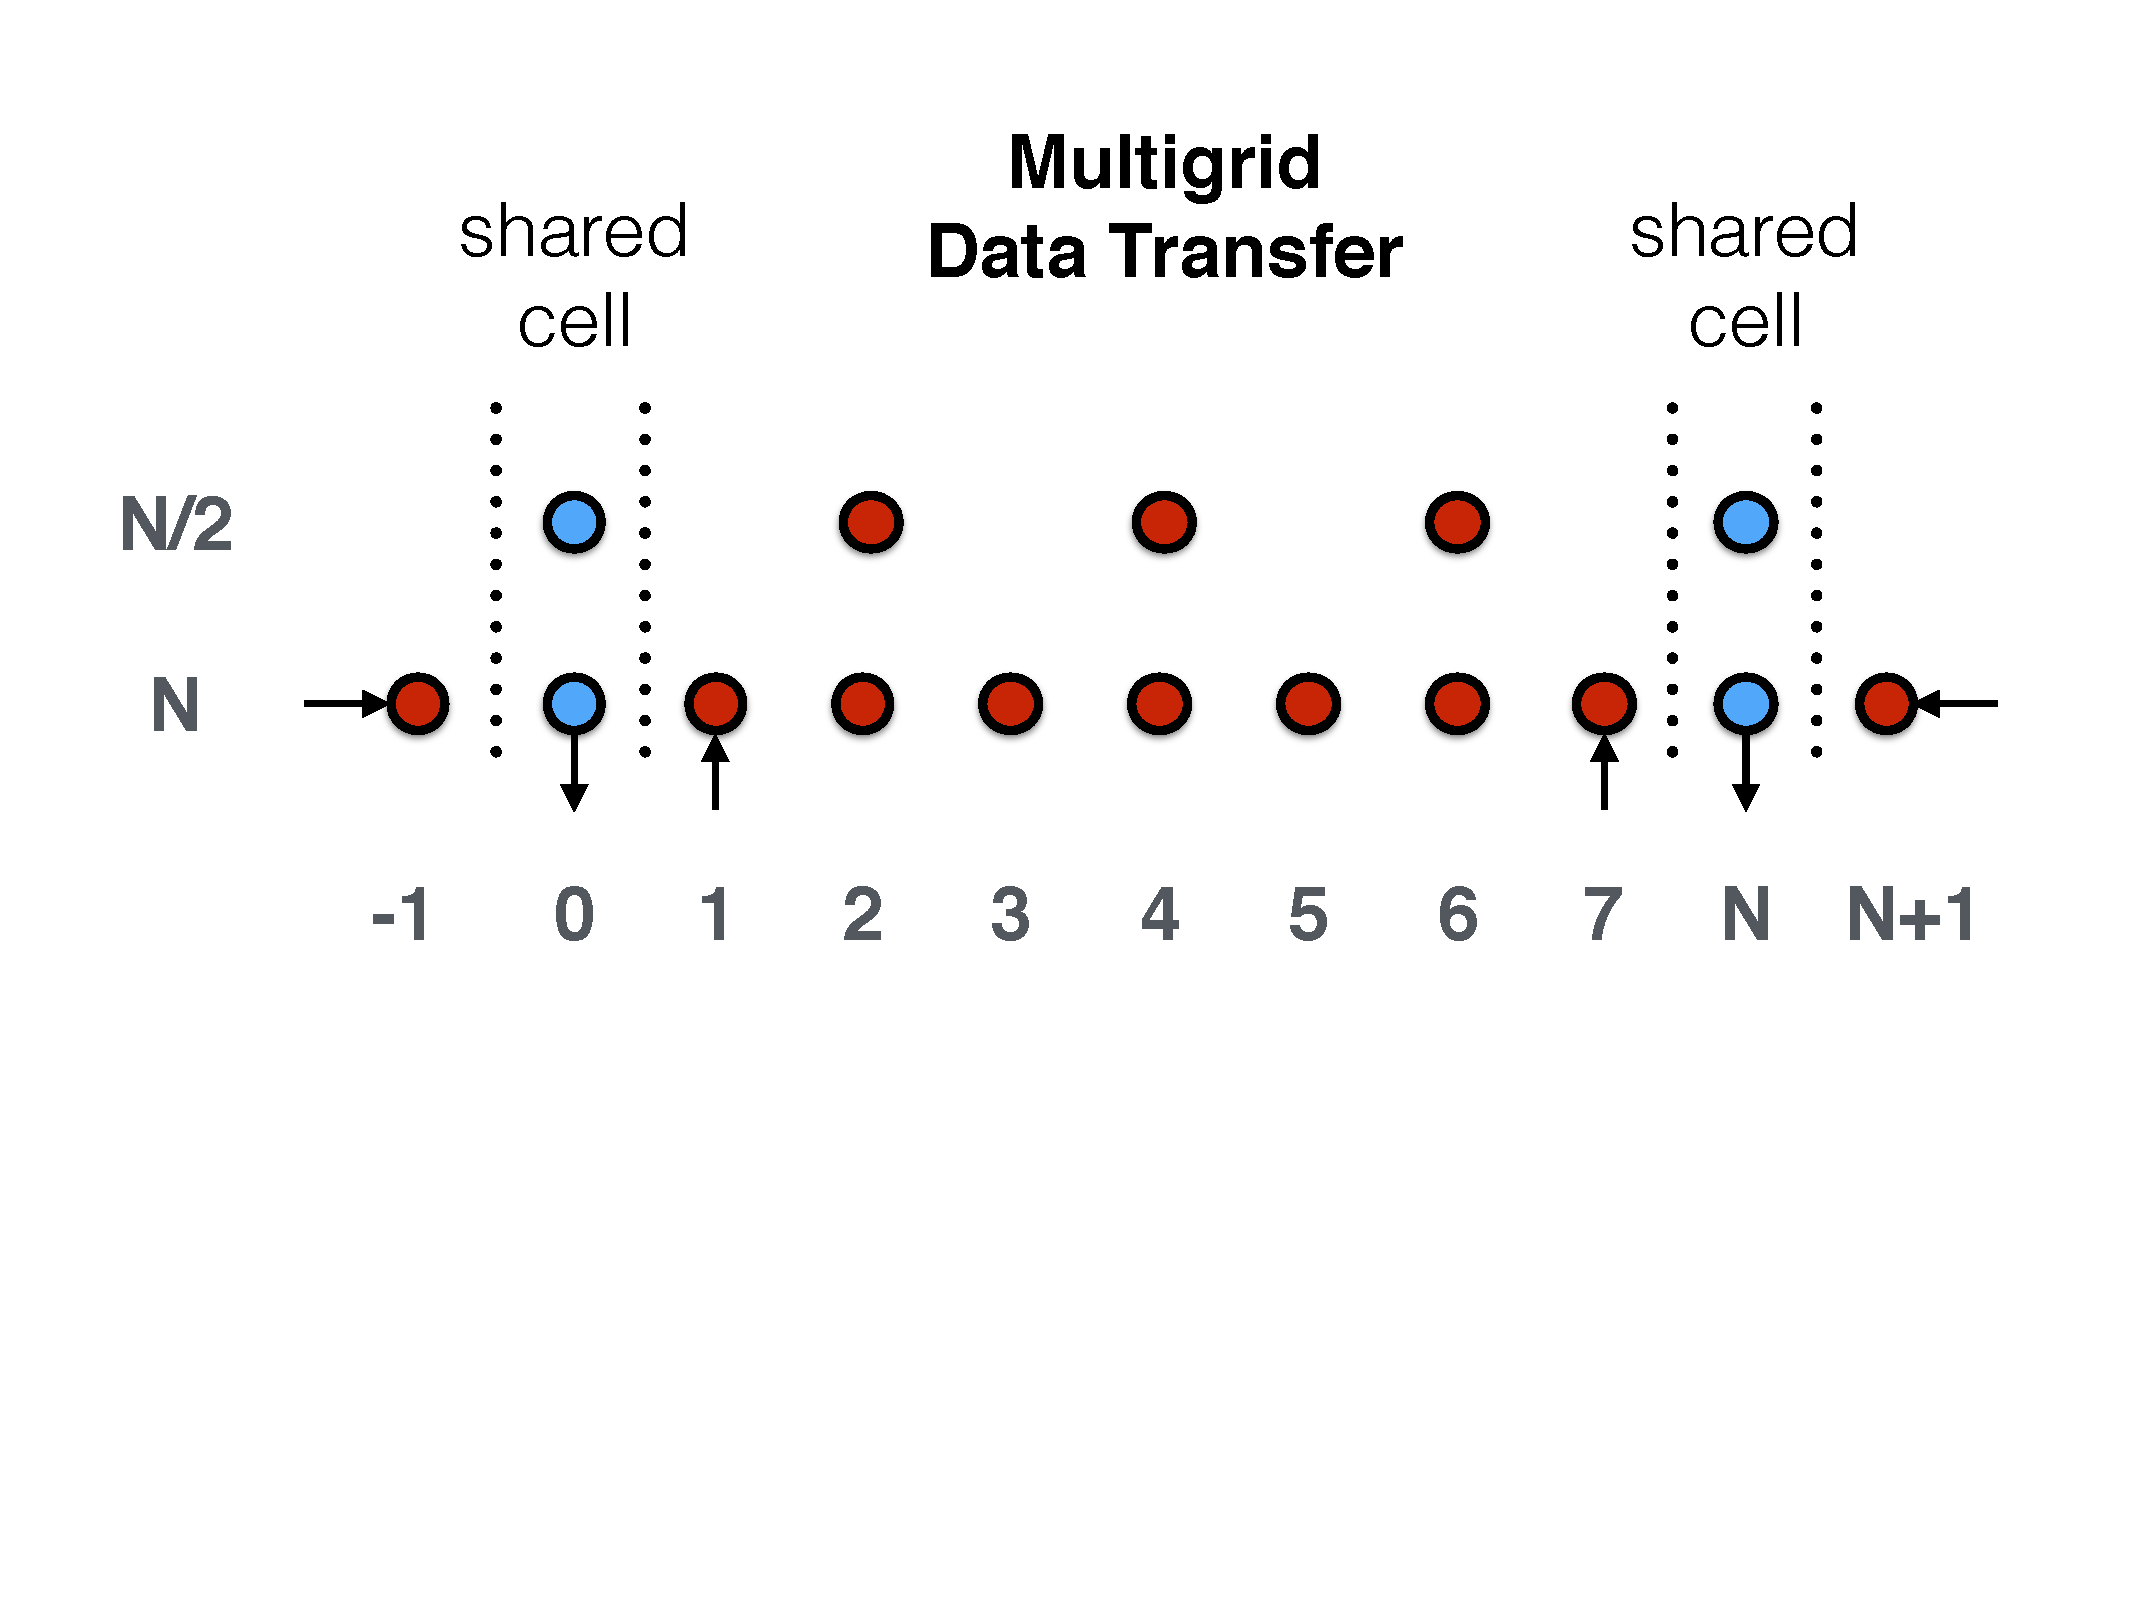
\includegraphics[width=2.5in]{Fig1}
\caption{Two multigrid levels (N,N/2) on one image showing the two cells that are shared with
  neighbors on the left and the right and computed redundantly.  The fine level grid (N)
  also shows the two cells that must be exchanged between neighbors.  Arrows represent the direction
  of data exchange from the perspective of the local image.}
\label{fig_grids}
\end{figure}

Two levels of the grid hierarchy are shown in Fig. \ref{fig_grids} running on a processor computing on
an interior portion of the grid; additional images are computing on regions to the left and right of
the region shown in the figure.  The finest grid (size N) is shown
in the bottom of the figure with cell indices running from (-1:N+1).  Cells 0 and N are shared
between image neighbors to the left and right (indicated by the light blue coloring and the vertical
dashed lines).  These shared cells are computed redundantly on each program image.

The red cells in the figure are computed concurrently on all subimages (one per image).
This distribution of computation over the hierarchical domain of images and subimages
requires communication of boundary regions between the various computational resources.
The communication is shown by arrows in the grid level N of the figure.  Data in cells 1
and 7 must be transferred from the subimage (upwardly pointing arrows) and the shared cell
computations must be copied to the subimage (downwardly pointing arrows). The horizontal
arrows represent data computed and subsequently transferred from the left and right
neighbors.

\begin{figure}[!t]
\centering
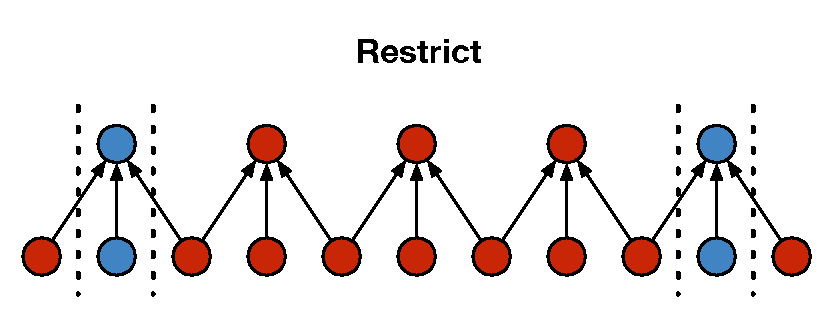
\includegraphics[width=2.5in]{Fig2}
\caption{Restriction of fine grid to coarse grid. Arrows show the points used in
         mapping onto the coarse grid.}
\label{fig_restric}
\end{figure}

The second grid level N/2 is also shown in Figure \ref{fig_grids}.  Data on this grid is obtained
by simple interpolation from information on grid level N as shown in Figure \ref{fig_restric}.
We call this interpolation a restriction and refer the reader to previous work on the multigrid
technique for more information\cite{multigrid_methods}.  The approximate solution on the N/2
grid is relaxed a few times and then passed on to grid level N/4 for further iteration.

\begin{figure}[!t]
\centering
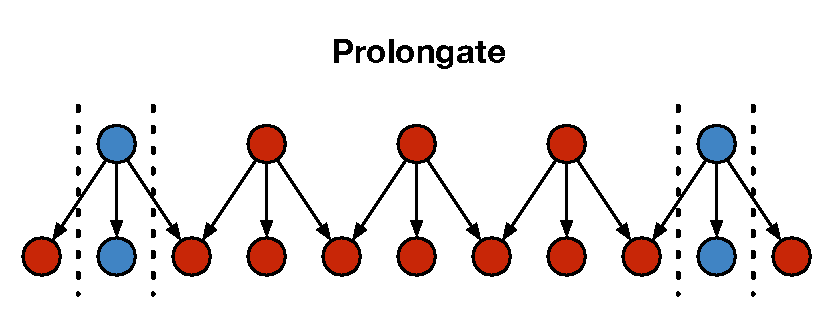
\includegraphics[width=2.5in]{Fig3}
\caption{Prolongation of coarse grid to fine grid. Arrows show the points used to
         interpolate onto the fine grid.}
\label{fig_prolongate}
\end{figure}

At the top of the grid hierarchy there are sufficiently few cells that an exact solution can be
obtained (perhaps by a non-iterative method).  This solution is then propagated down the
grid hierarchy as shown in Figure \ref{fig_prolongate}.

\subsection{Implementation of the Relaxation Step}

The multigrid algorithm has been implemented in Fortran using the CAFe
syntax described in the previous section. Data coarrays at each grid
level are declared, allocated, and initialized on each program image.
These coarrays are then copied to the subimages by the parent, hosting
images.  Below we show the implementation of the relaxation loop on
grid level N.  Each iteration step incorporates concurrent computation
on an image and its hosted subimage.  In order to execute
concurrently, we must declare an event variable to allow concurrent
execution and then synchronization once computation on \emph{both} 
the subimage \emph{and} the image have completed.

The event variable is declared as,
%%\small
\begin{verbatim}
 type(event_type) :: evt
\end{verbatim}
%%\normalsize
After initialization, this event variable has its count variable set to 0 and is incremented
each time the subimage task completes during an iteration of the code segment shown below:

\vskip 20pt

\small
\begin{verbatim}
 do i = 1, nsteps                            1
   call relax (N, V1h[dev], Buf[dev])        &
                    [[dev, EVENT=evt]]       2
   call relax_boundary (N, V1h)              3

   wait event (evt, until_count=i)           4

   V1h(0)[dev] = V1h(0)                      5
   V1h(N)[dev] = V1h(N)                      6

   V1h(  1) = V1h(  1) [dev]                 7
   V1h(N-1) = V1h(N-1) [dev]                 8

   sync all                                  9

   V1h( -1) = V1h(N-1) [left]               10
   V1h(N+1) = V1h(  1) [right]              11

   sync all                                 12
 end do                                     13
\end{verbatim}
\normalsize

This example shows the first relaxation steps on the finest grid level N.  The initial
guess (provided by the coarray \texttt{V1h}) is relaxed \texttt{nsteps} times as
specified by the loop beginning at statement 1.  The relaxation is computed on
the subimage \texttt{dev} by the call to the \texttt{relax} procedure at statement 2.
This call uses coarray memory located on the subimage as specified by the arguments
\texttt{V1h[dev]} and \texttt{Buf[dev]}, where the second coarray is used for temporary
storage.

Since an event \texttt{evt} has been supplied to the call in statement 2, the program
continues execution without waiting for the remote task on \texttt{dev} to complete.  The
count associated with the event will be increased by an implicit post to the event once
the task has finished executing.  Thus the task started by statement 2 will execute
concurrently with the \texttt{relax\_boundary} call at statement 3 --- the first call
executes on the subimage \texttt{dev} while the second call executes on the local image
\texttt{this\_image()}.

Most of the computation is accomplished by the subimage executing the \texttt{relax}
procedure (not shown) operating over the interior corresponding to fine grid indices (1:N-1).
Concurrently, \texttt{relax\_boundary} operates on the boundary indices 0 and N
(note that memory for the boundary computation is located on local image as
the coarray \texttt{V1h} is not coindexed using square bracket notation in statement 3.

Once relaxation of the boundary has completed, the program image will wait for the event
indicating that the subimage task has finished executing relaxation on the interior (statement
4).  The \texttt{until\_count} for the event is increased by 1 each iteration of the loop,
so the program waits until the event counter equals the iterate counter \texttt{i}.

Once the wait has completed, communication of the halo regions between the subimage and
the hosting image can begin.  Shared boundary cells at 0 and N are copied \emph{to} the
subimage by the execution of statements 5 and 6 and interior regions at cells 1 and N-1 are
copied \emph{from} the subimage by statements 7 and 8.  Boundary cells are exchanged (copied)
from neighboring images by statements 10 and 11.  To ensure that no race conditions are
introduced by the exchange of information between images, explicit synchronization is
accomplished by the execution of statements 9 and 12.

\begin{comment}
There are four points to note regarding this memory allocation: 1. Memory is only allocated if a
subimage has been obtained; 2. The location where memory is allocated is denoted by regular coarray
notation \texttt{U[device]}; 3. The allocated size and halo attribute of the new array are obtained
from the previously allocated local array \texttt{U} via the notation \texttt{HALO\_SRC=U} (using
\texttt{HALO\_SRC} will also initially copy \texttt{U} to the subimage); and finally 4. The
allocation itself is \emph{executed} on the subimage device with the notation \texttt{[[device]]}.

Fortran uses square bracket notation, e.g. \texttt{[image]}, to specify on what process the
memory reference is physically located.  Square brackets are a visual clue to the
programmer that the memory reference may be remote and therefore potentially suffer a
performance penalty.  CAFe extends this by employing double-bracket notation to indicate
possibly \emph{remote subimage execution}.

Note that a transfer of halo memory is necessary after each completion of the do concurrent loop.
This must be done in order for the halo region of a coarray on a given process to be consistent
with the corresponding interior of the coarray on a logically neighboring process.
Finally, memory for the entire array \texttt{U} can be copied from the
subimage device with the statement,
\texttt{U = U[device]}, 
and memory deallocation (not shown) is similar to memory allocation.
\end{comment}

\section{Performance Measurements}

It is important to note that the emphasis of this work is to explore and explain the new
syntax and execution semantics of a CAFe application.  A thorough examination of potential
performance gains (if any) using CAFe for parallelization of code is beyond the scope of
this paper.  The primary purpose of CAFe is to combine the parallel features of Fortran coarrays
--- executing a \emph{single} program --- with concurrent execution of separate tasks executing on
potentially heterogeneous hardware.

\begin{comment}
However, the relative performance of computation on a cluster of GPUs compared with the
necessary communication of halo information is of interest, especially considering that a
complete exchange of halo data involves communication between multiple coarray images
\emph{and} between each individual host image and its subimage (an attached OpenCL
device).
\end{comment}

However the relative performance of computation on the interior of a three-dimensional
grid, performed by the GPU, compared with the time required to compute on boundary planes by the
CPU is of interest.  Table 1 shows average execution time for a relaxation step on the GPU
(column 2) and on the CPU (column 3) in milliseconds, where $N$ (column 1) is the number of
cells in one dimension of a 3D cube; time for the exchange of halo information
between the GPU and the CPU for each iteration is also shown in column 4.

\begin{table}[]
\centering
\caption{Size of cube and time in milliseconds}
\label{table1}
\begin{tabular}{rrrrr}
$N$   &   GPU	 &  CPU         &   Comm    \\
      &   	 &              &           \\
16    &  0.02    &   0.01	&   0.07    \\
32    &  0.02    &   0.03       &   0.10    \\
64    &  0.04    &   0.12       &   0.27    \\
128   &  0.42    &   0.47	&   0.81    \\
256   &  4.59    &   1.97	&   2.99    \\
512   & 43.08    &   12.51	&  16.49    \\
\end{tabular}
\end{table}

Note that all three times in Table 1 are roughly equivalent for $N=128$.  Also note that
the communication and the computational times on the CPU are roughly equivalent and scale
the same with increasing $N$.  This is not surprising as both involve only the surface
elements of the cube.  However, computational time on the GPU grows much faster, O($N^3$),
as it is computing on the interior of the cube.

\begin{comment}
The current implementation does \emph{not} take advantage of optimization strategies such
as prefetching of array tiles (including halos) into OpenCL local memory.  Neither does it
take advantage of the potential of CAFe to overlap communication with computation (for
example, computing on ...
\end{comment}

\begin{comment}
Since many scientific codes are dominated by memory performance, including and especially
stencil algorithms as they typically only involve a computation on a small locally central
array element and a small overlapping halo region.  Stencil operations frequently do not
contain enough floating point operations per memory load to allow for floating point
performance to operate at peak (though this is entirely application and domain specific).
Thus we illustrate the \emph{potential} for performance by noting the latency and
throughput performance of an attached GPU in conjunction with MPI distributed memory
performance associated with halo transfer in Table 1.
\end{comment}

\begin{comment}
The results in Table 1 indicate that the primary bottleneck in using accelerators attached
to the TODO bus using OpenCL is likely to be the latency in transferring memory to and
from the device for distributed memory clusters of only a few nodes exchanging halo data
using MPI.
\end{comment}


\section{Conclusions}

Fortran is a general-purpose programming language and is extremely important to the
scientific and high performance computing (HPC) community.  While new code development is
often in languages other than Fortran, such as C++, Fortran usage in terms of CPU hours on
HPC platforms remains as high as ??? \cite{Yellick::language:breakdown}.  Fortran will be
with us well into the future as the lifetime of important scientific applications is
measured in decades and Fortran usage dominates in scientific communitities that are
critical to understanding the future of life on our planet such as the climate community.

However significant challenges arise as hardware adapts to the end of Moore's
Law\cite{exascale:workshop:2011}.  The revolution occurring in the hardware architecture
has completely altered the landscape for scientific computing as a code designed for
distributed memory bulk synchronous model of parallelism may actually run slower on
advanced hardware\cite{Dubey:2014:SSC:2686745.2686756}.

Parallelism was added to Fortran with the addition of coarrays in the 2008
standard\cite{fortran:2008} to enable the migration of codes as hardware evolves.
Significant language features were left out of this early version of coarrays as
identified by \emph{Mellor-Crummy et al}\cite{mellor-crummey:2009:caf2}.  Many of these features
have been adopted in what is likely to be called the 2015 standard of the language\cite{fortran:2015},
such as teams of program images and improved synchronization constructs like events.
However, the Fortran coarray model fails to address heterogeneity in hardware as is already
being seen in HPC computing platforms with the adoption of distributed nodes consisting of
general purpose CPUs with attached accelerator devices like GPUs, for example, in the early
RoadRunner Machine at Los Alamos\cite{RoadRunner} and new machines arriving such as Blue
Waters\cite{blue:waters}.

Current


In this preliminary work we have examined ....
In no way does this represent a thorough examination of these potential features.

CAFe introduces the concept of subimages executing on a hosting image.  CAFe includes
\item
  Dynamic creation of subimages.
\item
  Dynamic memory allocation and placement on a subimage.
\item
  Explicit addressing of memory on subimages using standard coarray notation.  It follows
  the Partitioned Global Address Space model (PGAS), although with subimages the address
  space is hierahical in the sense that the memory partioning only allows memory exchange
  between a subimage and its hosting image as initiated by the hosting image.
\item
  Task creation and execution on subimages using extended coarray syntax with double
  square brackets \testtt{[[ ]]}.  Task mays be defined in terms of standard \emph{pure}
  Fortran procedures and task execution continues without interuption until completion.
  In addition a Fortran 2015 event may be notified upon completion of the task to allow
  concurrent execution on the subimage and on the hosting image.
\item
  CAFe integrates Fortran 2015 features to allow relatively simple programs to be written
  that employ all of the heterogenous components expected on exascale platforms.

\subsection{Limitations}

Possible criticism of this work includes the following:
\item
  The source-to-source transformations that have been developed to implement CAFe
  are rudimentory and have not been optimized.  For example, memory transfers have
  not been aggregated into larger messages to improve performance.  Memory transfer
  is also blocking so that prefetching of data cannot be employed via techniques
  envolving the reordering of statements (code motion) that effectively employed in
  CAF compilers.
\item
  The Laplacian example is in reality a ``toy'' problem.  Real multiphysics codes
  employ hundreds of more variables and would have entirely different performance
  characteristics because of the increased pressure on cache and register usage.
\item
  Existing scientific codes often separate communication into separate modules from
  the computational kernels.  This makes adoption of CAF itself slow (because these
  MPI modules already work fine) and thus additional extensions like CAFe also
  would be slow to adopt. However CAFe constructs can be used in an incremental
  fashion making it easier to adopt
\item
  In reality CAF (and therefore CAFe) are relatively low-level parallel programming
  languages that require the programmer to \emph{explicitly} control the placement
  of memory, communication, and synchronization.  Perhaps higher level languages like
  Chapel would be better to adopt as they could provide an easier programming model
  to the programmer and possibly more avenues for compiler optimization.
\item
  Thorough examination of performance capabilities on real scientific applications
  (or at least scientific ``mini-apps'') has not been attempted.
\item
  Programming models like that proposed by CAFe already exist in the form of a combination
  of MPI and OpenMP (or OpenACC) programs.  The advantage of CAFe --- by being a purely
  language construct --- is that it opens up the possibility of compiler optimizations
  that would otherwise be impossible with a library approach intermixed with compiler directives.

\subsection{Future Work}

However, especially with the integration of task-based parallelism with synchronization
events arriving in Fortran 2015, the possibilities are intriguing.  Tasks plus the
dependencies represented by events suggest a correspondence with the Open Community
Runtime (OCR) libraries.  In OCR, the entire program must be broken into a set of tasks
represented by a directed acycic graph (DAG).  In OCR, tasks are available for executing
when all of their input dependencies are satisfied, such occurs when computation of a new
interation of data elements have been updated and other upstream tasks have completed.

Tools to automatically convert existing codes to run under the OCR model faces challenges.  For
example, the hundreds of MPI functions would have to be semantically understood by the tools,
integrated with existing OpenACC directives (for example), a DAG generaged for the complete
program, and then transformed into an OCR program.

An intriguing \emph{possibility} exists for automatic conversion of CAFe codes to OCR exists:
\item
  CAF codes have well defined boundaries (called segment boundaries) indicating where new
  OCR tasks must be created.
\item
  CAF has many fewer library routines (primarily collectives) that must be converted.
\item
  CAF has events which already define some of the dependencies necessary for the creation
  of OCR tasks.
\item
  CAFe introduces the notion of task based parallelism (in addition to the existing
  Fortran features like \texttt{do concurrent}.

In the future we hope to examine \emph{if} the possibility exists for CAFe codes to be
automatically converted to programs employing the Open Community Runtime.

\begin{comment}
These choices often hide the opportunity for
optimizations by the compiler \cite{Dubey:2014:SSC:2686745.2686756}.
\end{comment}

%
% This could be part of conclusions
%

%%Note that the use of halo cells is the normal way that large and complex MPI and CAF programs are implemented.

\subsubsection{Benefits.}
LOPe proposes to formalize the common, halo software pattern in language syntax, thus providing the
compiler with access to halo information in order to spread computation over more hardware
resources, improve performance, and to reduce complexity for the programmer.  Furthermore, LOPe
semantics provide important \emph{language restrictions} that remove the possibility of race conditions
that occur when multiple threads have write access to overlapping data regions.

\subsubsection{Limitations.}
LOPe only supports regular structured grids through Fortran multi-dimensional arrays and a
corresponding multi-dimensional processor layout.  It does not allow the composability of stencils
required by non-linear physics operators, nor does it provide automatic support for the storage of
intermediate results resulting from multiple intermediate update steps.  Adaptive Mesh Refinement
(AMR) Shift Calculus provides a generalized abstraction that addresses many of these concerns
(see\cite{Dubey:2014:SSC:2686745.2686756} and references therein).  However, it may be possible to
support AMR in LOPe through locally-structured grid methods based on the work of Berger and
Oliger\cite{colella2007performance}.  In this instance, LOPe could be used to update the regular
array regions in each rectangular patch.

By implementing LOPe we have demonstrated that LOPe can be used to easily and succinctly code
the stencil algorithms that are common to many areas of science, and furthermore, that LOPe is
suitable for transformation to languages like OpenCL that support heterogeneous computing.  It
remains to history to ascertain if LOPe is sufficiently general purpose to be included in a
general-purpose programming language or if it is better suited to remain as a DSL and to be used as a
special-purpose preprocessing tool.


% conference papers do not normally have an appendix

% use section* for acknowledgement
\section*{Acknowledgment}

This work was supported in part by the Department of Energy Office of Science, Advanced Scientific
Computing Research.  The authors would also like to thank Robert Robey and Wayne Weseloh at Los
Alamos National Laborabory for several stimulating conversations with respect to programming models.



% An example of a floating figure using the graphicx package.
% Note that \label must occur AFTER (or within) \caption.
% For figures, \caption should occur after the \includegraphics.
% Note that IEEEtran v1.7 and later has special internal code that
% is designed to preserve the operation of \label within \caption
% even when the captionsoff option is in effect. However, because
% of issues like this, it may be the safest practice to put all your
% \label just after \caption rather than within \caption{}.
%
% Reminder: the "draftcls" or "draftclsnofoot", not "draft", class
% option should be used if it is desired that the figures are to be
% displayed while in draft mode.
%
%\begin{figure}[!t]
%\centering
%\includegraphics[width=2.5in]{myfigure}
% where an .eps filename suffix will be assumed under latex, 
% and a .pdf suffix will be assumed for pdflatex; or what has been declared
% via \DeclareGraphicsExtensions.
%\caption{Simulation Results}
%\label{fig_sim}
%\end{figure}

% Note that IEEE typically puts floats only at the top, even when this
% results in a large percentage of a column being occupied by floats.


% An example of a double column floating figure using two subfigures.
% (The subfig.sty package must be loaded for this to work.)
% The subfigure \label commands are set within each subfloat command, the
% \label for the overall figure must come after \caption.
% \hfil must be used as a separator to get equal spacing.
% The subfigure.sty package works much the same way, except \subfigure is
% used instead of \subfloat.
%
%\begin{figure*}[!t]
%\centerline{\subfloat[Case I]\includegraphics[width=2.5in]{subfigcase1}%
%\label{fig_first_case}}
%\hfil
%\subfloat[Case II]{\includegraphics[width=2.5in]{subfigcase2}%
%\label{fig_second_case}}}
%\caption{Simulation results}
%\label{fig_sim}
%\end{figure*}
%
% Note that often IEEE papers with subfigures do not employ subfigure
% captions (using the optional argument to \subfloat), but instead will
% reference/describe all of them (a), (b), etc., within the main caption.


% An example of a floating table. Note that, for IEEE style tables, the 
% \caption command should come BEFORE the table. Table text will default to
% \footnotesize as IEEE normally uses this smaller font for tables.
% The \label must come after \caption as always.
%
%\begin{table}[!t]
%% increase table row spacing, adjust to taste
%\renewcommand{\arraystretch}{1.3}
% if using array.sty, it might be a good idea to tweak the value of
% \extrarowheight as needed to properly center the text within the cells
%\caption{An Example of a Table}
%\label{table_example}
%\centering
%% Some packages, such as MDW tools, offer better commands for making tables
%% than the plain LaTeX2e tabular which is used here.
%\begin{tabular}{|c||c|}
%\hline
%One & Two\\
%\hline
%Three & Four\\
%\hline
%\end{tabular}
%\end{table}


% Note that IEEE does not put floats in the very first column - or typically
% anywhere on the first page for that matter. Also, in-text middle ("here")
% positioning is not used. Most IEEE journals/conferences use top floats
% exclusively. Note that, LaTeX2e, unlike IEEE journals/conferences, places
% footnotes above bottom floats. This can be corrected via the \fnbelowfloat
% command of the stfloats package.


% trigger a \newpage just before the given reference
% number - used to balance the columns on the last page
% adjust value as needed - may need to be readjusted if
% the document is modified later
%\IEEEtriggeratref{8}
% The "triggered" command can be changed if desired:
%\IEEEtriggercmd{\enlargethispage{-5in}}

% references section

% can use a bibliography generated by BibTeX as a .bbl file
% BibTeX documentation can be easily obtained at:
% http://www.ctan.org/tex-archive/biblio/bibtex/contrib/doc/
% The IEEEtran BibTeX style support page is at:
% http://www.michaelshell.org/tex/ieeetran/bibtex/
%\bibliographystyle{IEEEtran}
% argument is your BibTeX string definitions and bibliography database(s)
%\bibliography{IEEEabrv,../bib/paper}
%
% <OR> manually copy in the resultant .bbl file
% set second argument of \begin to the number of references
% (used to reserve space for the reference number labels box)

\bibliographystyle{IEEEtran}
\bibliography{cafe}{}


%\begin{thebibliography}{1}
%\bibitem{IEEEhowto:kopka}
%H.~Kopka and P.~W. Daly, \emph{A Guide to \LaTeX}, 3rd~ed.\hskip 1em plus
%  0.5em minus 0.4em\relax Harlow, England: Addison-Wesley, 1999.
%\end{thebibliography}




% that's all folks
\end{document}


